% This is a sample LaTeX input file.  (Version of 12 August 2004.)
%
% A '%' character causes TeX to ignore all remaining text on the line,
% and is used for comments like this one.

\documentclass{article}      % Specifies the document class

\def\Course{Principles of Computer System Design}
\def\Exam{Exam}
\def\Studentname{Tudor Dragan (xlq880)}
\def\Sub_date{\today}
                             % The preamble begins here.
%\title{\bf Principles of Computer Systems Design\\ {\Large Exam}}  % Declares the document's title.
%\author{Tudor Dragan\\}

\title{\Course\\\Exam}
\author{\Studentname}
\date{\Sub_date}      % Deleting this command produces today's date.

\usepackage{verbatimbox}
\usepackage{listings}
\usepackage{color}
\usepackage[]{amsmath}
\usepackage[english]{babel}
\usepackage[utf8]{inputenc}
\usepackage{graphicx}
\usepackage{moreverb}
\usepackage{hyperref}
\usepackage[T1]{fontenc} % font
\usepackage{program}
\usepackage[top=1.5in, bottom=1.5in, left=1.4in, right=1.4in]{geometry}
\usepackage[super]{nth}
\usepackage{fancyhdr}
\usepackage{lastpage}
\definecolor{dkgreen}{rgb}{0,0.6,0}
\definecolor{gray}{rgb}{0.5,0.5,0.5}
\definecolor{mauve}{rgb}{0.58,0,0.82}

\lhead{\textbf{\Course}}
\rhead{\Exam~(Submission: \Sub_date)}

\cfoot{}
\lfoot{\Studentname}
\rfoot{\thepage\ of \pageref{LastPage}}
\pagestyle{fancy}
\renewcommand{\footrulewidth}{0.4pt}


\lstset{frame=tb,
      language=Java,
      aboveskip=3mm,
      belowskip=3mm,
      showstringspaces=false,
      columns=flexible,
      basicstyle={\small\ttfamily},
      numbers=none,
      numberstyle=\tiny\color{gray},
      keywordstyle=\color{blue},
      commentstyle=\color{dkgreen},
      stringstyle=\color{mauve},
      breakatwhitespace=true
      tabsize=3
}
\newcommand{\ip}[2]{(#1, #2)}
                             % Defines \ip{arg1}{arg2} to mean
                             % (arg1, arg2).

%\newcommand{\ip}[2]{\langle #1 | #2\rangle}
                             % This is an alternative definition of
                             % \ip that is commented out.

\begin{document}             % End of preamble and beginning of text.

\maketitle                   % Produces the title.


\section*{Question 1: Data Processing} 

\subsection* {1. Sort-based external memory algorithm}

\begin{figure}[htbp]
\begin{center}
\begin{lstlisting}
//TODO: Insert pseudocode here
\end{lstlisting}
\caption{Sort-based external memory algorithm}
\label{Sort-based external memory algorithm}
\end{center}
\end{figure}

For this part of the exam we must implement an algorithm that first applies an aggregated function (in our case the \emph{count} function) on the table \emph{friends}, and then combine the results to write up the table that consists of (uid, networh, nrOfFriends). In order to achieve this, I used a modified sort-merge join algorithm.\\

I made the following assumptions:
\begin{enumerate}
\item
We don't have any indices on the tables so the entries are not in sorted order in any of the two tables.
\item  
The friends table has only uni-directional relations, in the sense that Person1 can be friends with Person2 but it's not requested that Person2 has to be friends with Person1. (Person1 has 1 friend and Person2 has 0 friends.)
\item
The table with the biggest number of records has \emph{N} records.
\item
We know that the main memory can hold \begin{math}\sqrt{N}\end{math} records. If we read B records at a time in memory, the number of runs will be \begin{math}N/B\end{math}.
\item 
Number of passes in Phase 2 is P then: \begin{math}B(B-1)^P = N\end{math}\\
 \end{enumerate}

First I build the table with the aggregate count function for the friends table by altering the way that we merge the pages on a pass. I will explain how it is done in the following paragraphs on a concrete example:

\begin{enumerate}
\item 
Every entry in the friends table has this form : ($uid1$, $uid2$). The input is split up in multiple blocks. Let us assume that we have a block that has these following ($uid1$, $uid2$) relations:
(3,7) (1,4) (2,3) (2,5) (1,3) (1,2) (2,4) (3,1)
\item
In order to calculate the number of friends for each user, I will sort records with the form ($uid1$, $friendCount$). because every record in the \emph{friends} table essentially means 1 friend added, when reading in the first phase, the $friendCount$ is 1. So we will have initially tuples with the form ($uid$, 1) that need to be sorted by \emph{uid}. We assume that the buffer page number is 4. So after the first phase we will have [(3,1) (1,1) (2,1) (2,1)] [(1,1) (1,1) (2,1) (3,1)]. 
\item
The next pass will be [(1,1) (2,2) (3,1)] [(1,2) (2,1) (3,1)], Then we combine the values by adding up the number of friends by comparing the heads of the lists (the heads contain the smallest $uid$) and add up or write to disk the smallest one $uid$ with the friend count.
\item
Finally we will have [(1,3) (2,3) (3,2)].
\item 
This will continue until all the pages buffers are empty and have no more data to fill them up with. 
\end{enumerate}

After we create the number of friends table that has entries sorted by $uid$, we sort the $user$ table We sort the users by uid because we would like to split both sorted inputs into blocks and combine the result to (uid, networh, nrOfFriends) output form. Because we have space in memory for \begin{math}\sqrt{N}\end{math} records, each buffer block should have a size of \begin{math}\sqrt{N}/2\end{math}. We compare the heads of the lists, because they always have the smallest possible id and merge the values together. We continue filling up the buffers and stop when there are no more entries to compare.
  
\subsection* {2. Hash-based external memory algorithm}

\begin{figure}[htbp]
\begin{center}
\begin{lstlisting}
//TODO: Insert pseudocode here
\end{lstlisting}
\caption{Hash-based external memory algorithm}
\label{Hash-based external memory algorithm}
\end{center}
\end{figure}

The hash-based algorithm is very similar to the \emph{GRACE hash join algorithm} with a slight modification that increments a counter for displaying the number of friends for each user. We make the following assumptions:

\begin{enumerate}
\item 
There are B-1 buckets, with B main memory buffers. These buckets will hold \begin{math}\sqrt{N}/2\end{math} records, where N is the highest of U and F. 
\item
The hashtable in the second phase is smaller than B-1 pages.
\end{enumerate}

We first partition both relations U (user table) and F (friend table) via a hash function into B-1 buckets. We read one partition at a time. We iterate through it and place the record in one of the buckets by the hashing the join attribute (in our case the $uid$). Then we can be sure that if tuples of U and F join, they will wind up in corresponding buckets $U_i$ and $F_i$ for some \emph{i}. After this phase we read a bucket of $U$ from disk and hash it using another function and construct the hash table in memory. Then we load in an buffer for $S_i$ and iterate through it. When we match the $uid$, we increment the $numberOfFriends$ counter in the hash table. When the buffer is empty, we write to disk the hash table with $(uid, networth, numberOfFriends)$ and load the next entries in the buffer.\\

\subsection* {3. I/O costs}


\subsubsection* {Sort-merge algorithm}

For the sort-merge algortihm the "expected" cost is:
\begin{equation}
Sort_U + Sort_F + (Pages_U + Pages_F)
\end{equation}

\subsubsection* {Hash-based algorithm}

\section* {Question 2: Distributed Transaction}

\subsection* {1. Local wait-for-graphs}
Conflict-serializability is defined by equivalence to a serial schedule (no overlapping transactions) with the same transactions, such that both schedules have the same sets of respective chronologically ordered pairs of conflicting operations (same precedence relations of respective conflicting operations).\\

A schedule is conflict-serializable if and only if it's precedence graph has no cycles. This is a graph of nodes and vertices, where the nodes are the transaction names and the vertices are attribute collisions. The local waits-for graphs on each node are:\\


\begin{figure}[ht]
\centering

{%
\setlength{\fboxsep}{5pt}%
\fbox{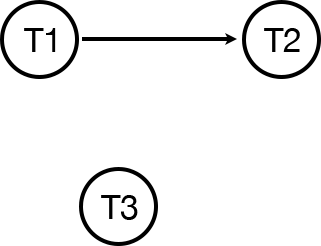
\includegraphics[scale=.3]{img/local-graph-1}}%
\fbox{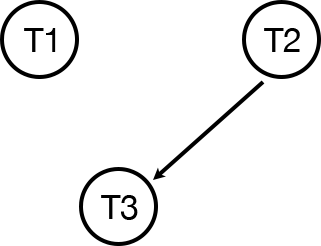
\includegraphics[scale=.3]{img/local-graph-2}}%
\fbox{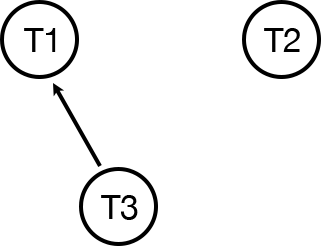
\includegraphics[scale=.3]{img/local-graph-3}}%
}%

\caption{Local wait-for-graph for Node 1, Node 2 and Node 3 \label{overflow}}
\end{figure}

As we can see the graphs have no cycles, proving that there are no local deadlocks.\\

\subsection* {2. Global wait-for-graph}

When constructing the global wait-for-graph we set up the pages that are being modified on each machine. If we have a cycle in the global graph, it means that we have conflicts and must abort the transactions. Below we have the global wait-for-graph: \\

\begin{figure}[ht]
\centering

{%
\setlength{\fboxsep}{5pt}%
\fbox{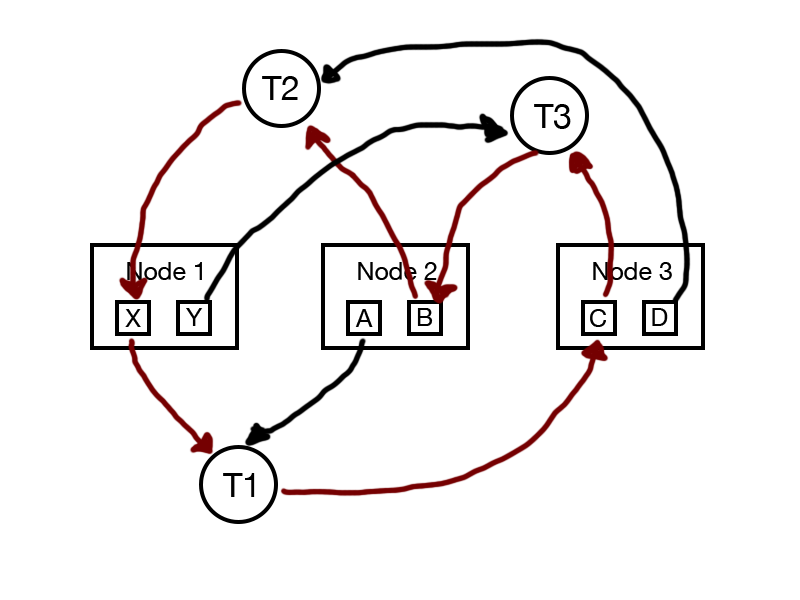
\includegraphics[scale=.3]{img/global-graph}}%
}%
\caption{Global wait-for-graph\label{overflow}}
\end{figure}

As we can see we have cycle between  $X -> T1 -> C -> T3 -> B -> T2 -> X$. To remove the deadlock within the system we must abort modifications that are being don on $X$, $C$ and $B$.

\end{document}               % End of document.